\section{Механика}
След като дефинирахме основно приближение в нашия, можем да преминем към изграждането на математическия
модел и последващото му решаване. Такъв един модел се поддава добре на разглеждане от гледна точка на
диференциалната геометрия. Физичният смисъл на това е, че се фокусираме върху взаимодействието на материални
точки (,,частици``) в рамките на апроксимацията на непрекъснатите среди (следствията от това приближение
ще бъдат дискутирани по-нататък в текста). 
Освен това ще бъдат разгледани само дисперсионните взаимодействия (т.нар $r^{-6}$ потенциал).

\begin{figure}[h]
    \centering 
    \subfigure[Схема на взаимодействието]{\label{fig:cylinder_front}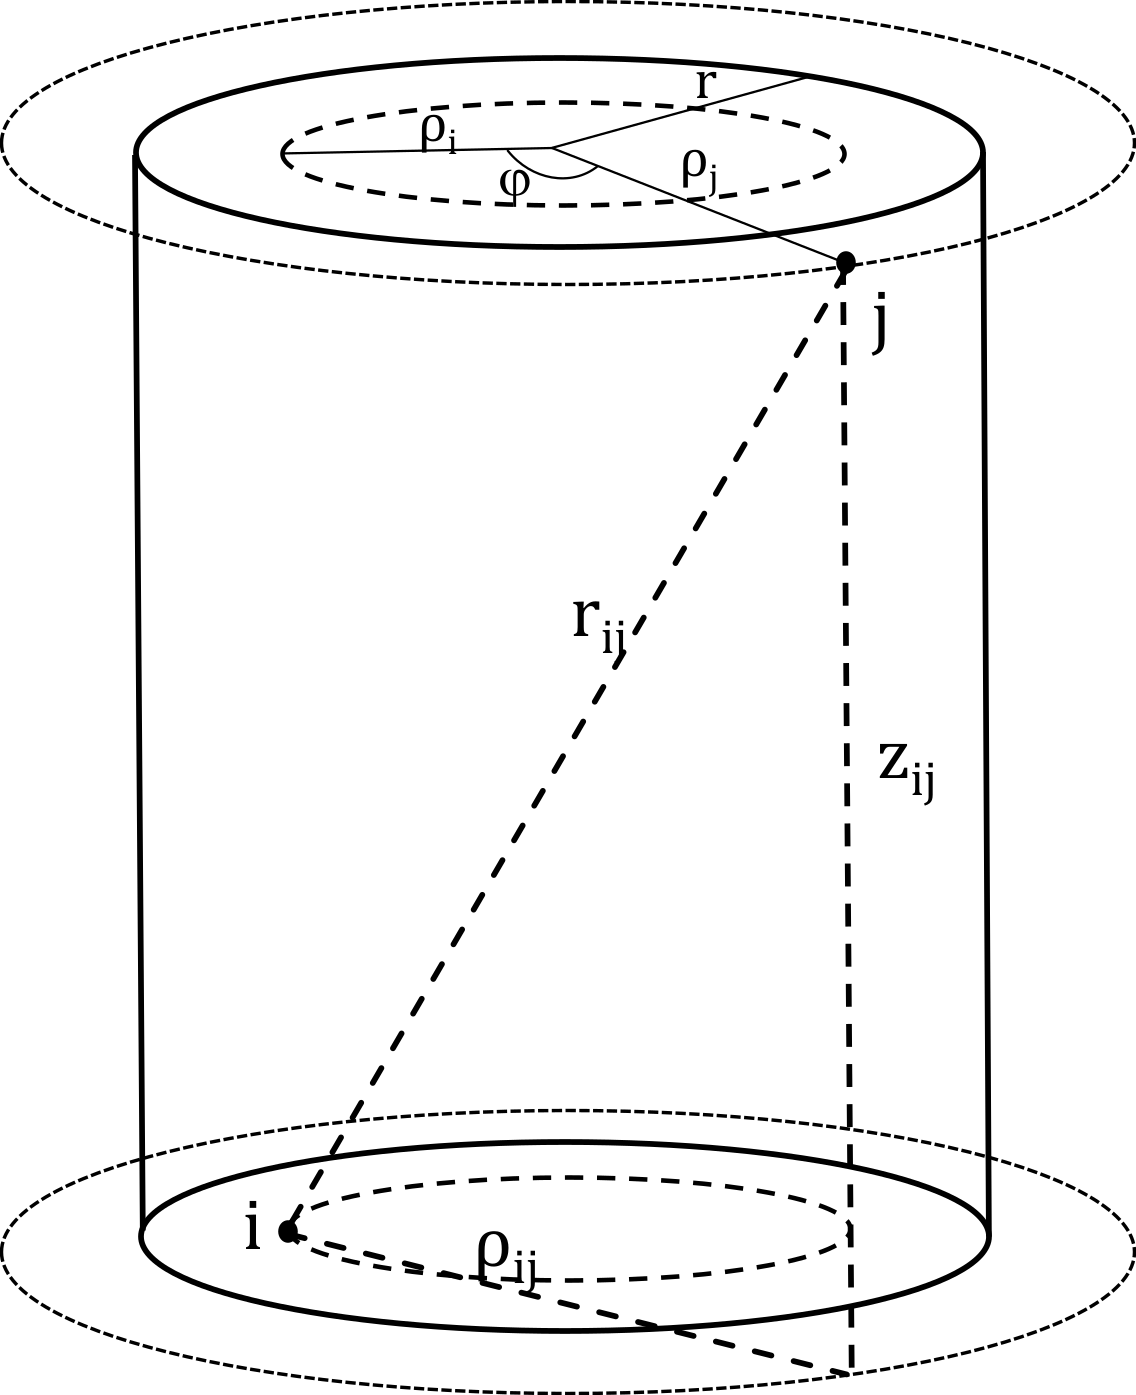
\includegraphics[width=0.48\linewidth]{cyl_fig_front.png}}
    \subfigure[Ортогонална проекция]{\label{fig:cylinder_top}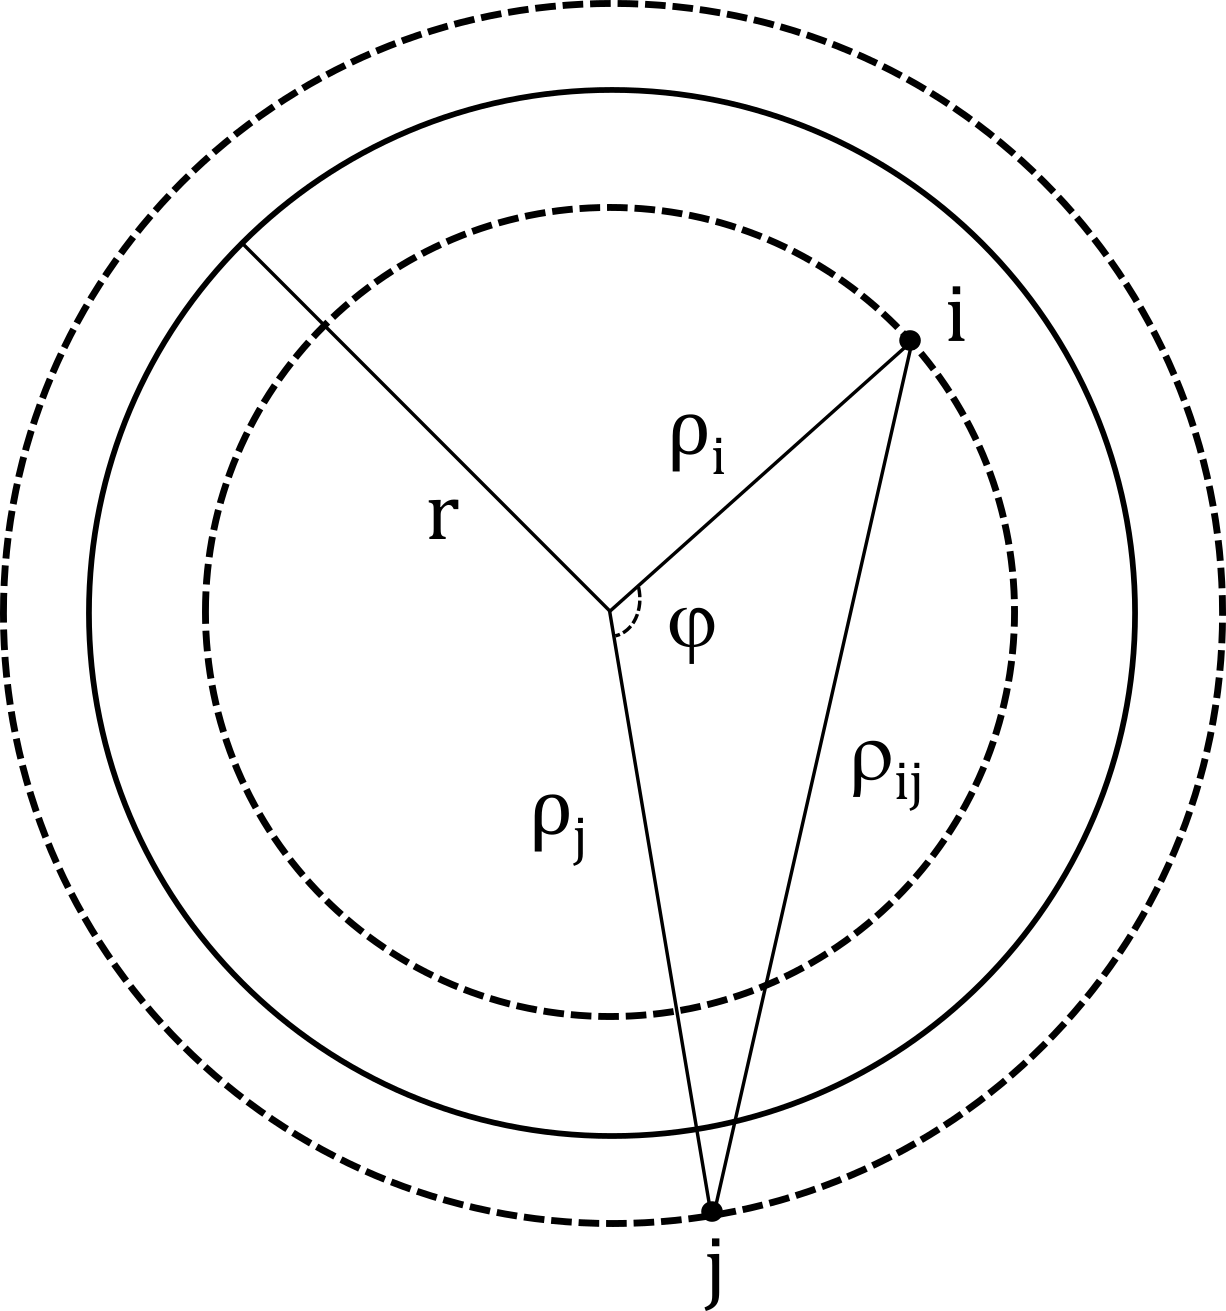
\includegraphics[width=0.48\linewidth]{cyl_fig_top.png}}
    \caption{
        Геометрична схема на разглежданата система. $r_{ij}$ - растояние между вътрешната \textbf{\textit{i}} и външната \textbf{\textit{j}} ,,частици``. $z_{ij}$ и $\rho_{ij}$ са съотвените проекции. $r_{ij}^2 = \rho_{ij}^2 + z_{ij}^2$. \textbf{\textit{r}} - радиус на цилиндъра.}
    \label{fig:cylinder_schematic}
\end{figure}

Такова разглеждания са правени много за случая на плоскопарелелните течни филми \cite{rusanov_shchekin}, като най-интересни са ,,тънките`` филми поради значителното влияние на капилярните
явления в тези системи. ,,Тънки`` (капилярни) са тези системи, чиито размери поне по едно от направленията са достатъчно малки, 
за да се наблюдава припокриване между двете междуфазови преходни области. В тях няма изотропен/обемен флуид, т.е. свойствата в тях са изцяло анизотропни. 
Всички ,,интересни`` капилярни явления всъщност са следствие от тази анизотропност на средата. 

Тук следва да отблежим, че механичния подход за тези системи е особено подходящ, тъй като в термодинамичния такъв губим детайлната информация за анизотропията - в случая на плоските филми
,,заместваме`` системата с опростена такава - обемен флуид ,,затворен`` между две математически равнини. От друга страна термодинамичния модел е удобен от практическа гледна точка - параметрите и енергиите
са адитивни. По тази причина оснвният ни анализ ще бъде механичен, а термодинамичните величини - напрежение на ,,филма``, повърхностно напрежение, разклинящо налягане и т.н. ще бъдат изведени като следствия
от получената по механичния подход енергия на взаимодействие.

\subsection{Получаване на енергията на взаимодействие}
Основна стъпка към анализа на система е получаването на плътността на енергията на взаимодействие между частиците. 
Дисперсионните взаимодействия имат адитивен характер \cite{israelachvili}, което ни позволява да представим нашата система като
,,потопена`` в един резервоар (в случая с безкрайни размери) или:
\begin{equation}
    w_{\infty}  = w + \tilde{w}
\end{equation}
Където $\tilde{w}$ е плътността на взаимодействието на елемент от разглежданата система \textbf{\textit{i}} ($0 < \rho_{i} < r$) (оградена от плътния контур на \autoref{fig:cylinder_schematic}) с елемент \textbf{\textit{j}} от съседната на цилиндъра част от безкрайна система ($r < \rho_{j} <  \infty$).
Безкрайния резервоар е по дефиниция хомогенен, т.е. неговата плътност на енергията е постоянна. Това позволява да заместваме съвсем просто енергията на цилиндъра с енергията на допълнителната система в уравненията, без загуба на обобщеност.
Още повече това ни позволява да останем в рамките на модела на непрекъснатите среди като избегнем работата с взаимодействия на къси разстояния, за които въпросния модел не е валиден, тъй като дискретната структура на системата започва да има силно отношение върху разглежданията.
В моделите, за да се избегнат сингулярности, се въвежда ,,най-малко разстояние`` $a$ (или нормирано към радиуса на цилиндъра $a_{c}$),
което стандартно се интерпретира като ,,молекулен диаметър``, макар че придаването на този физичен смисъл става \textit{a posteriori} \cite{israelachvili} и следва да се внимава 
при интерпретацията на резултатите за тези най-малки разстояния.


Според литературата  $\tilde{w_{i}} = (1/v_{m})^2 \int_{\tilde{V}}\epsilon_{ij}\,dv_{j}$ \cite{israelachvili}, където $\epsilon_{ij}$ е енергията на дисперсионното взаимодействие на частиците \textbf{\textit{i}} и \textbf{\textit{j}}, a $v_{m}$ - моларният обем на течността.
Съответно $\epsilon_{ij} = -\beta/(r_{ij})^6$, където $\beta$ е т.нар. Хамакерова константа, а $r_{ij}$ e праволинейното, евклидово разстояние между двете точки.
Тогава в декартови координати можем да запишем евклидовата норма:

\begin{equation}
    r_{ij}^2 = (x_{i} - x_{j})^2  + (y_{i} - y_{j})^2 + (z_{i}-z_{j})^2
    \label{eq:cartesian}
\end{equation}

Тъй като работим с цилиндрична симетрия, можем да направим преход към цилиндрични координати, като по конвенция:
\begin{align*}
    x &= \rho \cos(\phi) \\
    y &= \rho \sin(\phi) \\
    z &= z \\
    dV &= \rho \,d\rho \,d\phi \,dz
\end{align*}

Заместваме и опростяваме:
\begin{align*}
    r_{ij}^2 &= (\rho_{i}\cos(\phi_{i}) - \rho_{j}\cos(\phi_{j}))^2 + (\rho_{i}\sin(\phi_{i}) - \rho_{j}\sin(\phi_{j}))^2 + (z_i - z_j)^2 \\
    r_{ij}^2 &= (z_i - z_j)^2 + \rho_{i}^2 + \rho_{j}^2 - 2\rho_{i}\rho_{j}\cos{(\phi_i - \phi_j)}
\end{align*}

От тригонометричните равенства имаме:
\begin{align*}
    1-2 \sin{\left(\frac{x}{2}\right)}^2=\cos (x)
\end{align*}

Допълваме до точен квадрат и получаваме:
\begin{align*}
    r_{ij}^2 &= (z_i - z_j)^2 + \rho_{i}^2 + \rho_{j}^2 - 2\rho_{i}\rho_{j}\cos{(\phi_i - \phi_j)} \\
    r_{ij}^2 &= (z_i - z_j)^2  + (\rho_i - \rho_j)^2 + 4 \rho_i \rho_j \sin{\left( \frac{\phi_i-\phi_j}{2} \right)}^2
\end{align*}

В последното уравнение става ясно едно много важно следствие от симетрията - в цилиндрични координати експлицитни характеристики на двете точки са само техните разстояния от центъра на 
цилиндъра $\rho_{i}$ и $\rho_j$, а за останалите по две координати са важни само разликите. Т.е. ние директно можем да дефинираме:
\begin{align*}
    \hat{z_j} &= z_i - z_j \\
    \phi &= \phi_i - \phi_j \\
    \rho_{ij} &= (\rho_i - \rho_j)^2 + 4 \rho_i \rho_j \sin{\left( \frac{\phi_i-\phi_j}{2} \right)}^2
\end{align*}

Или финално:
\begin{equation}
    \label{eq:cylindricalcoords}
    r_{ij}^2 =  \hat{z_{j}}^2 + \rho_{ij}^2
\end{equation}

До същия резултат може да се достигне като се запише косинусовата теорема за триъгълника, който се формира при ортогоналната проекция на цилиндъра на \autoref{fig:cylinder_schematic}.
Концептуално това означава, че ние можем да опростим значително модела, тъй като цилиндърът може да се раздели на еквипотенциални равнини, перпендикулярни на $z$. Т.е. свеждаме задачата
до описанието на взаимодействието в една такава еквипотенциална равнина.

Готови сме да представим енергията, като изпускаме ,,материалните`` константи пред интеграла, тъй като основната цел е получаването на функционалната зависимост. Въпросните константи ще бъдат
определени и ,,възстановени`` след това.

\begin{equation}
    \label{eq:energy_integral_raw}
    \tilde{w_i} \displaystyle\propto \displaystyle\int_{r}^{\infty} \rho_{j} \,d\rho_{j} \displaystyle\int_{0}^{2\pi} \,d\phi \displaystyle\int_{-\infty}^{\infty} r_{ij}^{-6} \,d\hat{z_{j}}
\end{equation}

Интегрирането по $\hat{z_j}$ става лесно, тъй като $\hat{z_{j}}$ има независим от другите две координати принос в $r_{ij}$:
\begin{equation*}
    \displaystyle\int_{-\infty}^{\infty} r_{ij}^{-6} \,d\hat{z_{j}} = \frac{3\pi}{8} \rho_{ij}^5
\end{equation*}
Аналогичното интегриране по $\phi$ става след представяне на $\rho_{ij}$ в стандартната форма $\rho_{ij}^2 = (\rho_i - \rho_j)^2 + 4 \rho_i \rho_j \sin^2(\psi)$, където $2\psi=\phi$ \cite{gradshteyn}:
\begin{equation*}
    \displaystyle\int_{0}^{2\pi} \,d\phi/\rho_{ij}^5 = 4\Psi(p)/(\rho_j-\rho_i)^5
\end{equation*} 
Където:
\begin{align*}
    \Psi(p) &= \left. \left(2(2+p^2)\boldsymbol{E}(p/\sqrt{1+p^2}) - \boldsymbol{K}(p/\sqrt{1+p^2})\right)\middle/3(1+p^2)^{3/2}\right. \\
    \boldsymbol{E}(k) &= \displaystyle\int_{0}^{\pi/2} \sqrt{1-k^2 \sin^2(\phi)} \,d\phi \\
    \boldsymbol{K}(k) &= \displaystyle\int_{0}^{\pi/2} \frac{1}{\sqrt{1-k^2 \sin^2(\phi)}} \,d\phi \\
    p^2 &= (4 \rho_i \rho_j)/(\rho_j - \rho_i)^2
\end{align*}

Тъй като има известни неконсистентности в литературата по отношение дефиницията на пълните елиптични интеграли (най-вече по отношение на аргумента $k$), то в настоящата работа е използвана дадената по-горе, която съответно отговаря на на тази в \cite{gradshteyn}.

Така стигаме до последното интегриране - това по $\rho_j$. Тук преди това обаче, ще бъдат въведени две нормировки, които ще използваме широко нататък.
\begin{align*}
    x &= \rho_i/r && 0 \le x \le 1 \\
    \xi &= \rho_i/\rho_j
\end{align*}

И така, самият интеграл:
\begin{equation*}
    \rho_{i}^{-3} I(x) = \displaystyle\int_{r}^{\infty} \left. \Psi(p)\rho_j \,d\rho_j \middle/ (\rho_j-\rho_i)^5 \right.
\end{equation*}

И като краен резултат за енергията на взаимодействие получаваме:
\begin{equation}
    \tilde{w_i} = -C x^{-3} I(x) 
    \label{eq:energy_short}
\end{equation}
Където $ C = 3 \pi \beta / 2 v_{m}^2 r^3 $.
\begin{equation}
    I(x) = \displaystyle\int_{0}^{x} \frac{\Psi(p) \xi^2}{(1-\xi)^5}  \,d\xi
    \label{eq:energy_integral}
\end{equation}

Комбинацията от \autoref{eq:energy_short} и \autoref{eq:energy_integral} е нашето ,,мастър`` уравнение, което дава пълната информация за разглеждания модел.
И така, с този резултат физичната система изцяло е ,,преведена`` на езика на математиката. Тъй като обаче е видно, че този интеграл няма точно и директно решение в термините на прости, 
аналитични функции, то следващите фокусът на следващите параграфи ще бъде изцяло върху най-добрите методи за неговото приближено аналитично решаване. Численото му решение ще бъде използвано
единствено като ,,репер``, спрямо който да се оценяват въпросните приближения.
